% mnras_template.tex 
%
% LaTeX template for creating an MNRAS paper
%
% v3.0 released 14 May 2015
% (version numbers match those of mnras.cls)
%
% Copyright (C) Royal Astronomical Society 2015
% Authors:
% Keith T. Smith (Royal Astronomical Society)

% Change log
%
% v3.0 May 2015
%    Renamed to match the new package name
%    Version number matches mnras.cls
%    A few minor tweaks to wording
% v1.0 September 2013
%    Beta testing only - never publicly released
%    First version: a simple (ish) template for creating an MNRAS paper

%%%%%%%%%%%%%%%%%%%%%%%%%%%%%%%%%%%%%%%%%%%%%%%%%%
% Basic setup. Most papers should leave these options alone.
\documentclass[letters, usenatbib]{mnras}

% MNRAS is set in Times font. If you don't have this installed (most LaTeX
% installations will be fine) or prefer the old Computer Modern fonts, comment
% out the following line
\usepackage{newtxtext,newtxmath}
% Depending on your LaTeX fonts installation, you might get better results with one of these:
%\usepackage{mathptmx}
%\usepackage{txfonts}

% Use vector fonts, so it zooms properly in on-screen viewing software
% Don't change these lines unless you know what you are doing
\usepackage[T1]{fontenc}

% Allow "Thomas van Noord" and "Simon de Laguarde" and alike to be sorted by "N" and "L" etc. in the bibliography.
% Write the name in the bibliography as "\VAN{Noord}{Van}{van} Noord, Thomas"
\DeclareRobustCommand{\VAN}[3]{#2}
\let\VANthebibliography\thebibliography
\def\thebibliography{\DeclareRobustCommand{\VAN}[3]{##3}\VANthebibliography}


%%%%% AUTHORS - PLACE YOUR OWN PACKAGES HERE %%%%%

% Only include extra packages if you really need them. Common packages are:
\usepackage{graphicx}	% Including figure files
\usepackage{amsmath}	% Advanced maths commands
\usepackage{amssymb}	% Extra maths symbols

%%%%%%%%%%%%%%%%%%%%%%%%%%%%%%%%%%%%%%%%%%%%%%%%%%

%%%%% AUTHORS - PLACE YOUR OWN COMMANDS HERE %%%%%

% Please keep new commands to a minimum, and use \newcommand not \def to avoid
% overwriting existing commands. Example:
%\newcommand{\pcm}{\,cm$^{-2}$}	% per cm-squared

%%%%%%%%%%%%%%%%%%%%%%%%%%%%%%%%%%%%%%%%%%%%%%%%%%

%%%%%%%%%%%%%%%%%%% TITLE PAGE %%%%%%%%%%%%%%%%%%%

% Title of the paper, and the short title which is used in the headers.
% Keep the title short and informative.

\title[V4046\,Sgr high-resolution ALMA observations]{V4046\,Sgr high-resolution 1.3\,mm continuum ALMA observations: a disc with a thin ring}

% The list of authors, and the short list which is used in the headers.
% If you need two or more lines of authors, add an extra line using \newauthor
\author[R. Martinez Brunner et al.]{
R. Martinez-Brunner,$^{1}$\thanks{E-mail: rmartinezbrunner@gmail.com}
A. N. Other,$^{2}$
Third Author$^{2,3}$
and Fourth Author$^{3}$
\\
% List of institutions
$^{1}$Chile\\
$^{2}$Department, Institution, Street Address, City Postal Code, Country\\
$^{3}$Another Department, Different Institution, Street Address, City Postal Code, Country
}

% These dates will be filled out by the publisher
\date{Accepted XXX. Received YYY; in original form ZZZ}

% Enter the current year, for the copyright statements etc.
\pubyear{2020}

% Don't change these lines
\begin{document}
\label{firstpage}
\pagerange{\pageref{firstpage}--\pageref{lastpage}}
\maketitle

% Abstract of the paper
\begin{abstract}
   %%%%context
    V4046 Sgr is a nearby pre-main sequence spectroscopic binary system that has a gas-rich circumbinary disc.
    We report on new $\sim$20\,mas resolution Atacama Large Millimeter Array (ALMA) observations of the radio continuum at 1.3\,mm, and compare with archival SPHERE-IRDIS differential polarised imaging (DPI) of scattered-light at H-band (1.65\,$\micron$) to reach conclusions on the disc structure. We use a parametric a radiative transfer model of the circumbinary disc, computed with \textsc{radmc3d} to interpret the available data, including the spectral-energy-distribution, in terms of a physical model. In addition, we explore decompositions of the imaging data in polar coordinates to better constrain the disc radial structure. 
    We report a two ringed structure for the millimetre-size dust population with a narrow, less than 4.17$\pm$0.94\,au-wide inner ring located at 13.46$\pm$0.43\,au. 
    This ring is the finest reported so far in a gas rich protoplanetary disc. 
    The ring is surrounded by a $\sim$9\,au-wide gap, flanked by a very sharp outer ring starting at 24\,au. 
    %The radial profile of the outer ring exhibits an intriguing break at $\sim$35\,au. 
    The RT model reproduces accurately the available data.
    %We predict a three ringed structure for the small-dust population with a inner ring at $\sim$6\,au hiding under the coronagraph in the SPHERE observations. 
    %The shadow of the secondary reported previously from the scattered-light data is also reproduced by the RT model. 
    %The DPI image reveals strong forward-scattering at 1.65\,$\micron$, which we reproduced with rather large dust grains of no less than 0.4\,$\micron$, hinting at a deficit of very-small-grains. 
    Using the parametric model scale height as an estimated height, we found that the thin inner ring is stable.
    %Deeper ALMA observations may confirm the lopsided 5\,au ring.
    
 
%briefly describe the aims, methods, and main results
%single paragraph not more than 250 words
%No references should appear
\end{abstract}

% Select between one and six entries from the list of approved keywords.
% Don't make up new ones.
\begin{keywords}
 protoplanetary discs -- submillimetre: planetary systems -- radiative transfer
\end{keywords}

%%%%%%%%%%%%%%%%%%%%%%%%%%%%%%%%%%%%%%%%%%%%%%%%%%

%%%%%%%%%%%%%%%%% BODY OF PAPER %%%%%%%%%%%%%%%%%%


\section{Introduction} \label{sec:Introduction}

Recent observations of circumstellar discs have revolutionised the way we think about protoplanetary discs, but the focus of resolved imaging with the Atacama Large Millimeter Array (ALMA) or with VLT/SPHERE has been mainly been towards the brighter sources. This report is part of a survey of discs around T-Tauri Stars (DARTSS - ref Avenhaus, Perez et al in pret). Here, we present new 1.3\,mm continuum ALMA observation of V4046\,Sgr, which is a remarkable system where it is possible to observe fundamental processes associated with disc evolution.

V4046 Sagittarii (Sgr) is is a double-lined spectroscopic binary of a nearly equal-mass pair of K-type stars (K5 and K7) with masses of 0.90$\pm$0.05\,M$_{\sun}$ and 0.85$\pm$0.04\,M$_{\sun}$ \citep{Rosenfeld_2012} on a close ($a \approx 0.041$\,au), circular ($e\leq0.001$) orbit, with an orbital period of 2.42 days \citep{refId0}. The V4046\,Sgr system locate at 72.41$\pm$0.34\,pc \citep{Gaia}, and is a member of the $\beta$ Pictoris moving group \citep{Zuckerman_2004}, fixing its age at 23$\pm$3\,Myr \citep{Mamajek_2014}. V4046\,Sgr binary system is surrounded by a massive ($\sim$0.1\,M$_{\sun}$), gas-rich disc extending to $\sim$300\,au \citep{Rosenfeld_2013, Rodriguez_2010}. The disc has a vast variety of molecules with a detailed subarcsecond ALMA molecular line imaging study by \citet{Kastner_2018}. The chemical structure is composed of CO and HCN that display centrally peaked morphologies, a sequence of sharp and diffuse rings of complex nitrile group molecules (HC$_3$N, CH$_3$CN), deuterated molecules (DCN, DCO$^+$), hydrocarbons (C$_2$H) and others like N$_2$H$^+$, H$_2$CO.

To analyse the new ALMA data, we aim to reproduce the disc through a parametric model ran with the radiative transfer code \textsc{radmc3d} \citep{Dullemond_2012} so that the model would agree with the ALMA observation, a previous SPHERE-IRDIS observation and the Spectral Energy Distribution (SED). With the model representation of the dust density distribution and combined with a decomposition in polar coordinates of the ALMA image we can have better approximations of the radial structure of the disc. It is worth mentioning that previous models of V4046\,Sgr have been made \citep{Ru_z_Rodr_guez_2019, Rosenfeld_2013, 2019ApJ...882..160Q} but with the difference that our new reference observation of radio wavelengths has a sub-arcsecond resolution, allowing us to discover previously unseen underlying substructures of the large-dust grains disc. 

In the following sections, first we describe the new 1.3\,mm continuum observation alongside with a SPHERE-IRDIS \textit{H}-band image (Section \ref{sec:Observations}), present the structure of the parametric model used to simulate the disc (Section \ref{sec:model}), comment on the results of the comparison of the model with the data and a discussion of the main results (Section \ref{sec:results}). Finally, we share our main conclusions in Section \ref{sec:Conclusions}.

\section{Observations} \label{sec:Observations}

Disc structures can be explored by means of comparing mm continuum and scattered light images. These observations allow us to see the distribution of different populations of dust particles, while ALMA traces the millimetre-sized grains settled in the mid-plane of the disc, scattered light accounts for photons reflected off small micron-sized dust at the disc surface layer, high above the mid-plane. By comparing both we can determine whether asymmetries in scattered light correspond to surface ripples or deep structures intrinsic to the underlying density distribution. 

New ALMA observations of V4046\,Sgr were obtained in 2017 as part of the Cycle 5 program 2017.1.01167.S.. These were taken in the context of a larger survey for 14 optically visible TTauri discs at $\sim$50\,mas resolution. The survey simultaneously mapped 1.3\,mm continuum and the J = 2$-$1 line of $^{12}$CO with the C43-8 array configuration in band 6 (211-275\,GHz). In this work we focus exclusively on the data obtained in the 1.3\,mm continuum for our source, taken with a beam size of $0\farcs04 \,\times \, 0\farcs05$.

For this investigation we made use of previous polarimetric image (at 1.65$\micron$) taken at the ESO Very Large Telescope with the SPHERE-IRDIS instrument. A complete description of these image and all about data reduction was reported in \citet{Avenhaus_2018}. 

For our analysis of the ALMA image we used an image reconstruction strategy, using the non-parametric image synthesis of the \textsc{uvmem} package \citep{2006ApJ...639..951C, 2018A&C....22...16C} we can super-resolve the clean beam, obtaining an effective angular resolution $\sim$2-3 times higher than in the clean image with natural weights. The model obtains this higher resolution through fitting the data using Chi-squared minimisation. Here we adopted a pure $\chi ^2$ model image. The resulting \textsc{uvmem} image shown in Fig. \ref{fig:two} exhibits previously unseen substructure of the disc. This unique high-definition image reveals that the disc features a two-ring structure for the large grain dust with a broad gap between the rings. The wide and brighter outer ring has been observed in previous occasions, but the thin and weak inner ring has never seen before (\citet{Ru_z_Rodr_guez_2019} anticipated its existence). The outer ring has its peak intensity at $\sim$30\,au and reaches out to $\sim$60\,au. Additionally, we can observe that there is a surface brightness break at $\sim$35\,au, another feature that has never been considered.

\begin{figure*}
	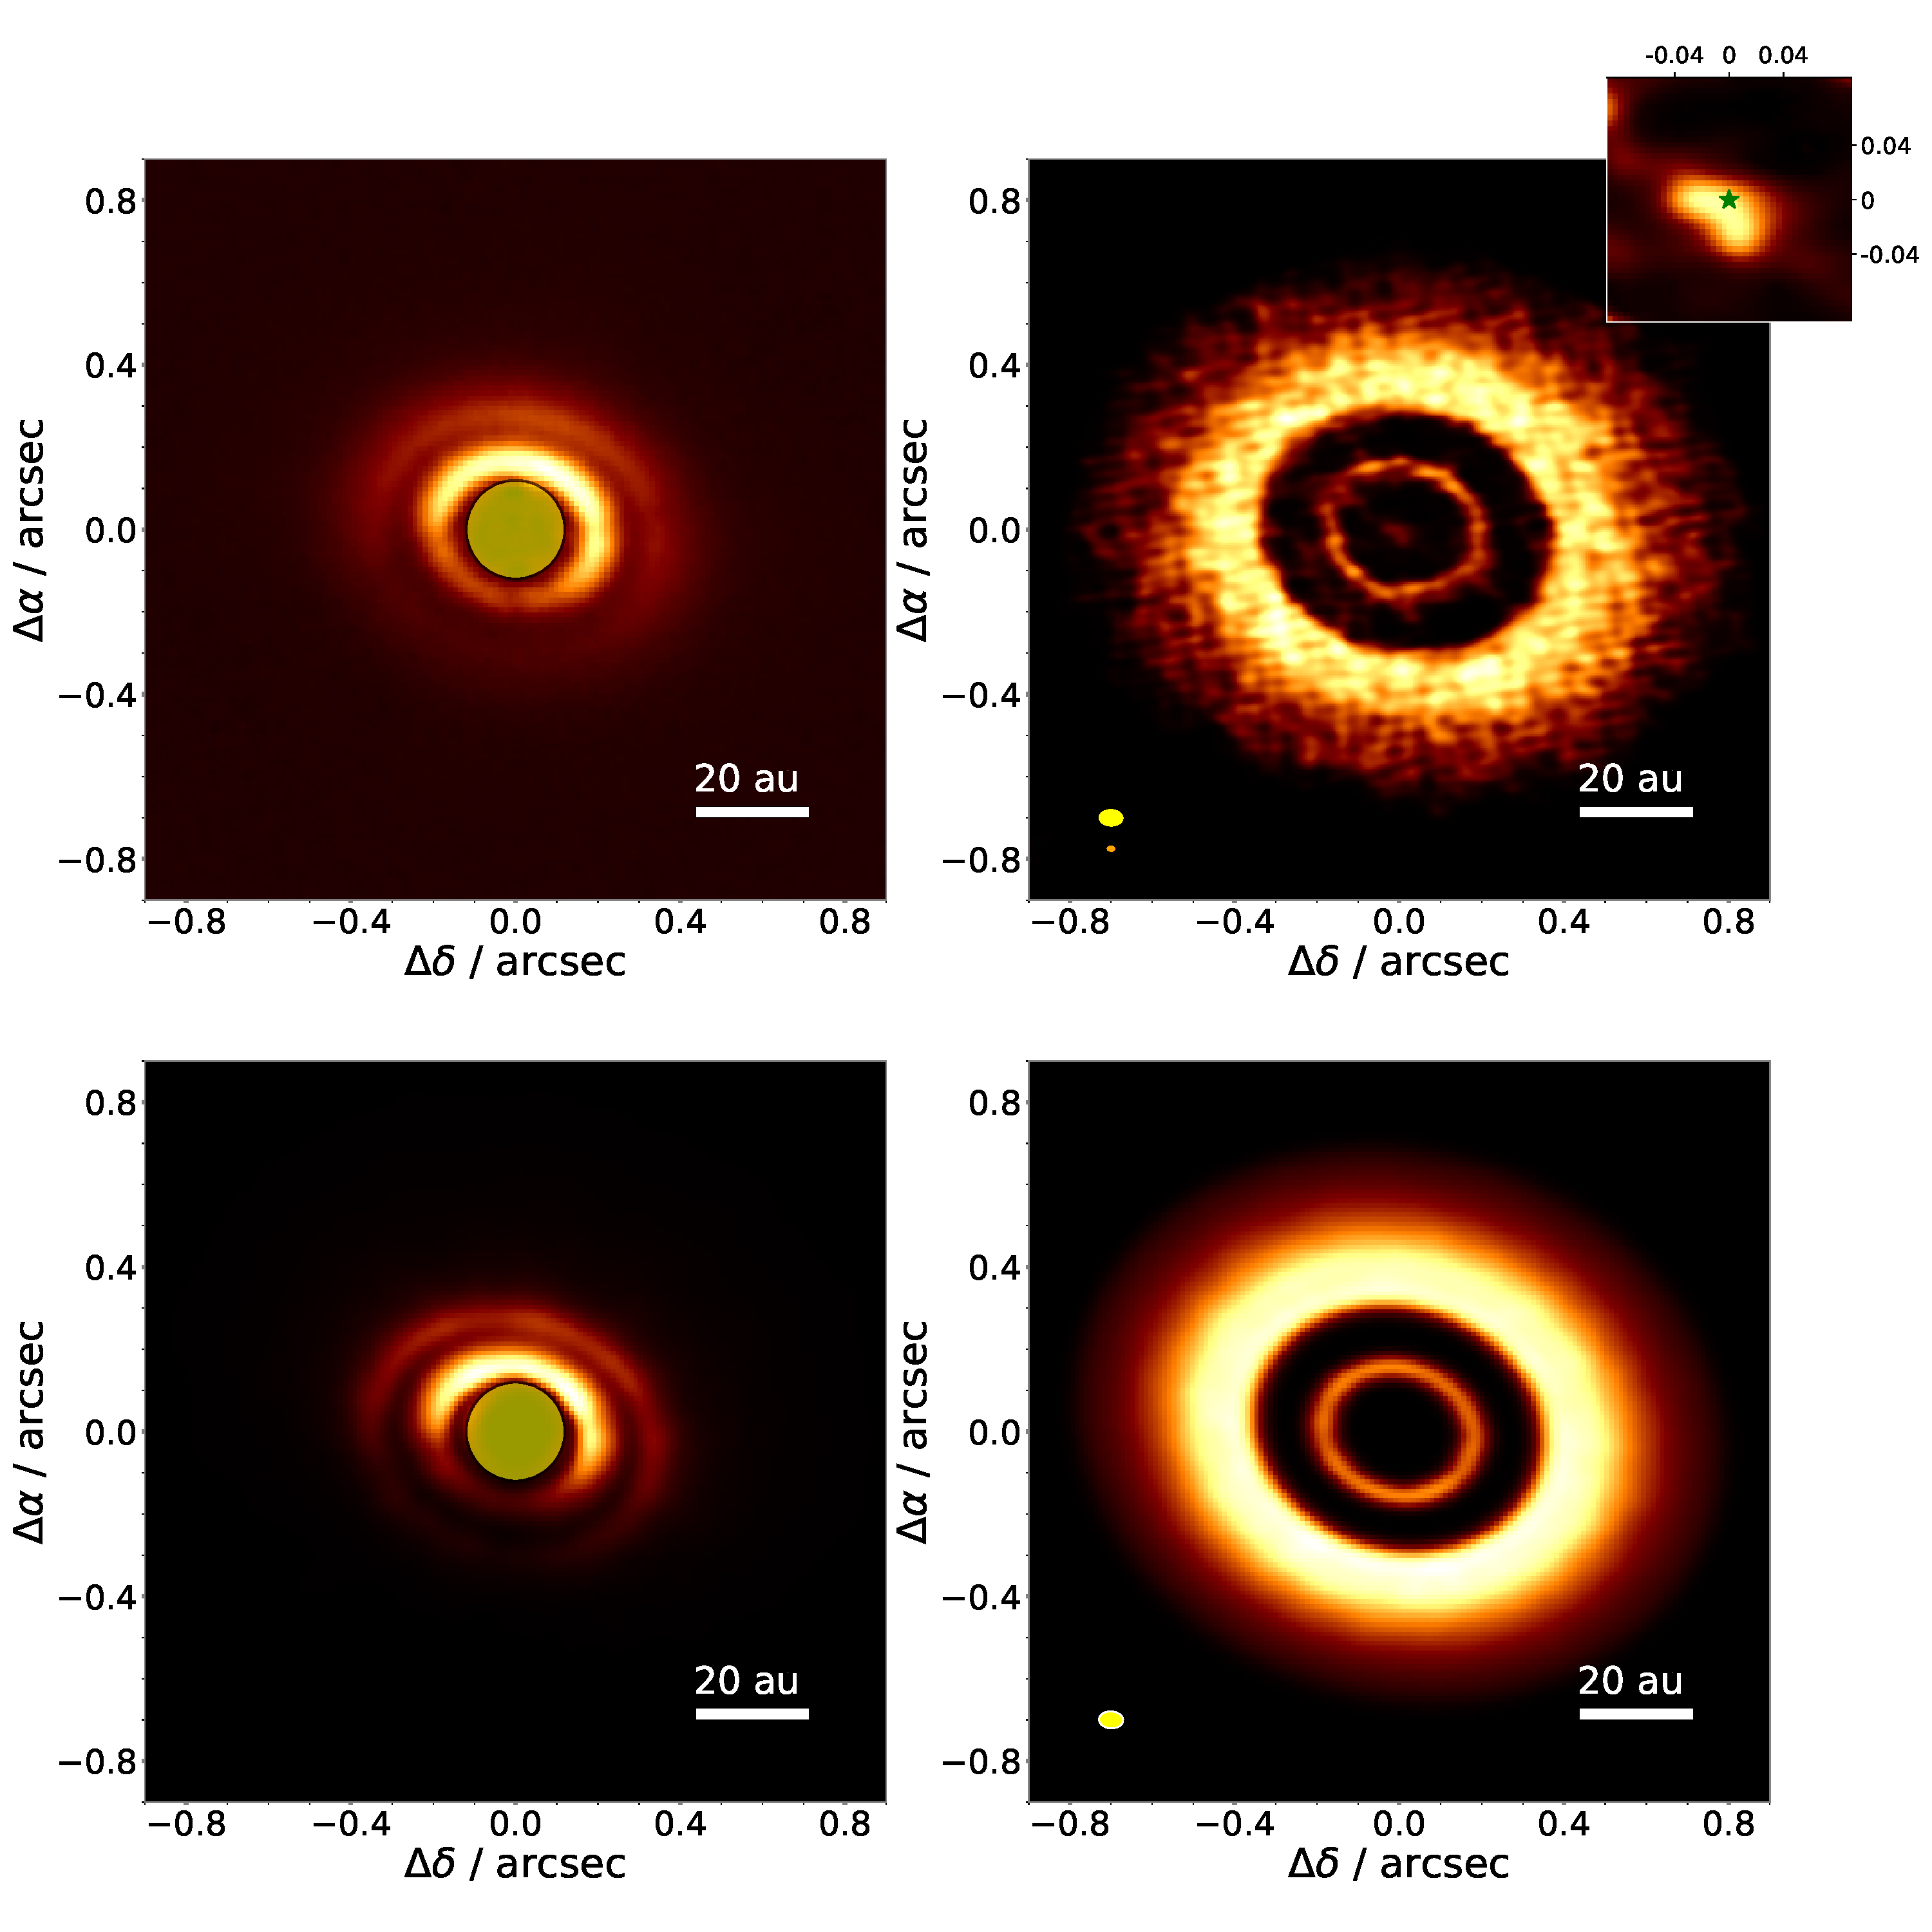
\includegraphics[width=\textwidth]{hot_two_E.pdf}
    \caption{Comparison of observations and simulated images at 1.65\,$\micron$ and 1.3 mm continuum of the circumbinary disc orbiting V4046\,Sgr. From top to bottom: DPI image and ALMA Band 6  observations; simulated images of the parametric model. Top left panel: SPHERE-IRDIS \textit{H}-band image with a yellow filled circle that illustrate the N\_ALC\_YJH\_S coronagraph (inner working angle $\sim0\farcs12$, or $\sim$8.6\,au at 72.4\,pc). Top right panel: 1.3\,mm continuum \textsc{uvmem} model image. The yellow ellipse shows the size of the natural-weighted beam: $ 0\farcs04 \, \times \, 0\farcs05$. The inset displays a enlarged view of the central emission, the green star marks the star positions. Bottom left panel: 1.65\,$\upmu m$ simulated image of the parametric model. Bottom right panel: 1.3\,mm simulated image of the parametric model. The yellow ellipse shows the size of the simulated beam: $ 0\farcs04 \, \times \, 0\farcs05$. For all the images in the figure the colour scale is linear.}
    
    \label{fig:two}
\end{figure*}

The inner ring is surprisingly narrow, and seems to be off-centre relative to the GAIA stellar position (at the origin of coordinates in Fig. \ref{fig:two}). The ring width can be measured in polar coordinates, following the determination of the inner ring centre and orientation. We minimised the dispersion of the disc radial profiles, from 6\,au to 19\,au (aiming for the inner ring) for a PA of 74.6\,$\degr$, an inclination of 33.9\,$\degr$ and a centre at $\Delta \alpha = 9\pm0.05$\,mas $\Delta \delta = 0.1\pm0.04$\,mas, relative to the stars. 

Assuming a Gaussian dust inner ring, we obtained the mean width and the location of the ring by finding for each azimuth the Gaussian intensity profile that best describes the ring. This gave us a FWHM of 4.17$\pm$0.94\,au and that it is located at 13.46$\pm$0.43\,au from the stars (See Fig. \ref{fig:polarring}). As we are using the \textsc{uvmem} model image and the effective angular resolution is $\sim$1/3 that of the natural-weighted beam ($0\farcs04 \,\times \, 0\farcs05$), these measurements only gives as an upper limit of the real width.

Doing one more time the minimisation of the dispersion of the disc radial profiles, but this time aiming for the outer ring from 20\,au to 70\,au, for a PA of 76.8\,$\degr$, with an inclination of 34.0\,$\degr$ and a centre at $\Delta \alpha = 19\pm0.04$\,mas $\Delta \delta = 7\pm0.03$\,mas relative to the stars, we can compare the measured location of the inner ring according with this parameters versus to the location obtained before. The deviation is shown in Fig. \ref{fig:polarring} and is not trivial since it depend on a few parameters such as the different inclinations of the rings, the difference in position angle and the small shifts of the centres relative to the stars. Those parameters play an important role, but a possible small difference in eccentricities between the inner and the outer ring could also help explain this deviation between the two measurements. ***

Interestingly, the ALMA images also detects faint the 1.3\,mm continuum near the stellar positions (See the inset in Fig. \ref{fig:two}). Since this faint central emission is offset from the star, at the origin of coordinates in the figure, it is probably due to large dust grains. This dust structure is at a distance of only $\sim0\farcs02$ from the binary system.

The scattered light image shown in Fig. \ref{fig:two} reveals the presence of a double ring structure in the micron-sized dust distribution. The observed morphology presents an inner cavity of $\sim$10\,au in radius and two rings located at 14.10$\pm$0.01 and 24.62$\pm$0.08\,au with a small gap between them at $\sim$20\,au. The observed second ring might correspond to the inner wall of the 1.3\,mm continuum emission outer ring \citep{Ru_z_Rodr_guez_2019}. Two other important features that are present in the image are: the brightness asymmetry and the shadows projected on the disc produced by the close binary system as they eclipse each other, described in detail by \citet{dOrazi}.

\citet{dOrazi} also measured the binary phase in the scattered light observation around 106\,$\degr$, setting $\phi=$0 from the North and increasing clockwise. We can then calculate the binary phase at the time of the ALMA observation at $\phi=$13\,$\degr$. There is no clear signal of any shadow similar to the ones present in the DPI image, this could be explained due to the slower cooling of larger grains (cite Casassus?***).

\begin{figure}
    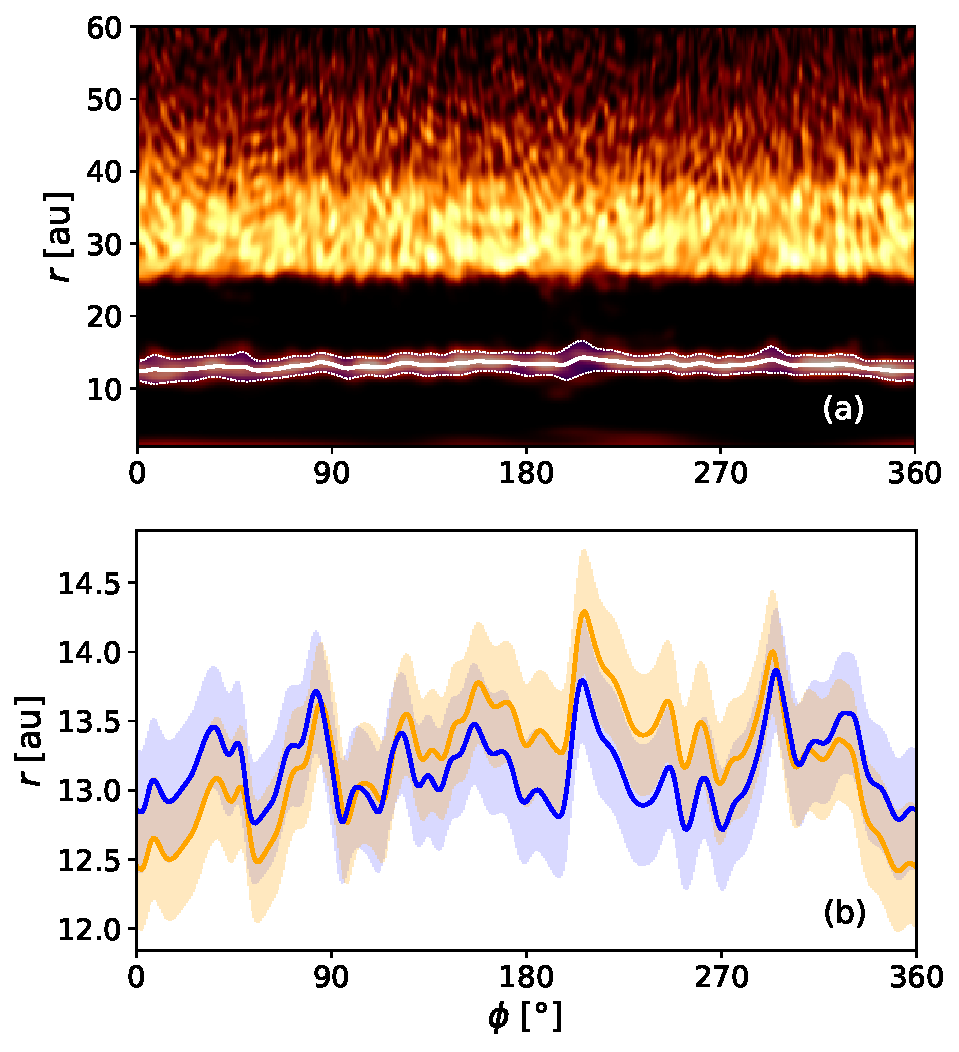
\includegraphics[width=\columnwidth]{polar_ring_aprox_and_diff_inner.pdf}
    \caption{(a) Polar decomposition of the 1.3\,mm continuum image showing the centres (solid line) of Gaussian fits and the measured FWHM (blue region between the dotted lines) of the inner thin ring for each azimuthal angle. This was obtained centring the \textsc{uvmem} image optimising for the outer ring. (b) Shows the measured location of the inner ring, where the orange line represents the centres of the fitted Gaussian profile obtained in the first panel and blue line represents the same but obtained centring the \textsc{uvmem} image optimising for the inner ring.}
    \label{fig:polarring}
\end{figure}

\begin{figure}
	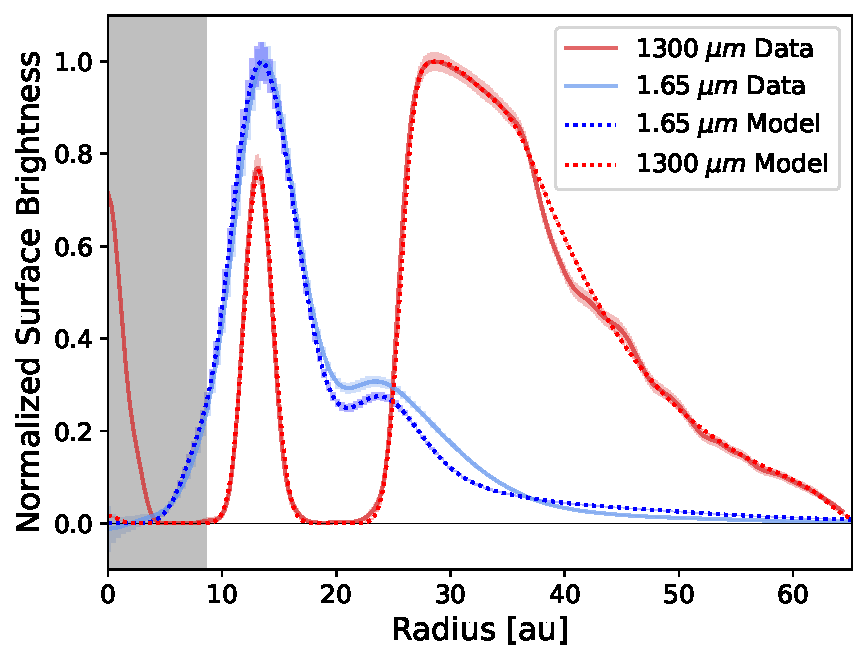
\includegraphics[width=\columnwidth]{comp_fig_all_profiles_au.pdf}
    \caption{Comparison of the surface brightness profiles extracted from the deprojected synthetic images and observed \textit{H}-band and 1.3\,mm continuum images. The grey shaded area represents the inner working angle of the artificial coronagraph used in the simulations (i.e., $\sim0\farcs 12$, or $\sim$8.6\,au at 72.4\,pc).}
    \label{fig:radprofiles}
\end{figure}

\section{Parametric radiative transfer model} \label{sec:model}

To search for a possible model that could explain the available data, we perform radiative transfer modelling with \textsc{radmc3d} \citep{Dullemond_2012}. Here we describe a 3D modelling framework for constructing disc structures given some parameters to characterise it. The model environment is similar to the one used by \citet{2018MNRAS.477.5104C} for DoAr 44. Through trial and error, we look for a set of values for the parameters that can define a model that correctly fits the available data.

For the representation of the stars we used two Kurucz photospheres models \citep{1979ApJS...40....1K, 1997A&A...318..841C} with  T$_{\mathrm{eff},1}=$ 4350\,K, R$_{*,1} =$ 1.064\,R$_{\sun}$, M$_{*,1} =$ 0.90\,M$_{\sun}$ and T$_{\mathrm{eff},2}=$ 4060\,K, R$_{*,2} =$ 1.033\,R$_{\sun}$, M$_{*,2} =$ 0.85\,M$_{\sun}$ respectively and with an accretion rate of log$\,\dot{\mathrm{M}}= -$9.3$\pm$0.3\,Myr$^{-1}$ for both cases. The stars were placed with a separation of 0.041\,au and arranged with a 30\,$\degr$ rotation to mach the shadows reported by \citet{dOrazi}.

Recreating the complex radial and vertical structure of the V4046\,Sgr disc is not an easy task. We choose to build the model by thinking the components of the disc separately and then unite them as a whole. Given the observations, we consider that a correct approach for this disc is using two different dust populations: larger grains that are vertically settled and dominates the disc mass and a less-abundant population of smaller grains that are distributed to larger heights from the mid-plane. As the gas and the small-dust population are coupled, it is important to consider the gas in the modelling process, but we are not predicting line emissions. 

Assuming a three dimensional model in a spherical reference frame with coordinates (r, $\theta$, $\phi$), gas density ($\rho_{\mathrm{gas}}$) distribution follows
\begin{equation}
  \rho_{\mathrm{gas}}(r,z) =\frac{\Sigma(r) \,\delta(r)}{\sqrt{2\pi} \,r H(r)}  \text{exp}\left[-\frac{1}{2} \left(\frac{z}{r H(r)}\right)^2\right].
\end{equation}
Where $\delta(r)$ is a parameter that indicates the density drops in the gaps and cavities, $H(r)$ is the scale height profile and $\Sigma(r)$ been the surface density profile. $\Sigma(r)$ is defined by
\begin{equation}
  \Sigma(r) = \Sigma_\mathrm{c} \left(\frac{r}{R_\mathrm{c}}\right)^{-\gamma}  \, \text{exp}\left[-\left(\frac{r}{R_\mathrm{c}}\right)^{2-\gamma}\right],
\end{equation}
where $R_c$ is a characteristic radius and $\gamma$ is the surface density gradient. We used a fixed $\gamma$ = 1, a typical value for discs \citep{Andrews_2009,Andrews_2010}. 

We define the parametric scale height profiles for the gas and for each dust population as \begin{equation}
    \label{scale}
  H(r)=\chi \, H_{o}(r) \, [r/r_{o}(r)]^{\psi(r)},
\end{equation}
where $H_o$ is the scale height at r = $r_o$, $\psi$ is the flaring index and $\chi$ is a scaling factor (in the range $0-1$) that mimics dust settling. For the gas and the micron-sized grains $\chi$ = 1 and for the millimetre-size dust population, as \citet{Rosenfeld_2013}, we assign a fixed $\chi$ = 1/2 for simplicity.

The small-dust density distribution follows the same behaviour as the gas but with different scaling factors: the dust-to-gas ratio ($\zeta$ = 0.047 as \citet{Rosenfeld_2013}), the mass fraction between small and large dust particles ($f_{\mathrm{mass}}$) and a $\delta(r)$ factor for fine tuning that depends on the radius. So it is
\begin{equation}
\rho_{\mathrm{small-dust}}(r,z)=\rho_{\mathrm{gas}}(r,z)\, f_{\mathrm{mass}} \, \delta(r) \: \zeta .
\end{equation}

Since the large-dust grains are less coupled to the gas, their distribution has some important differences. We leave a large inner cavity and added another scaling factor (or filter) to generate the larger gap between the rings. For the inner ring we use the same profile as the gas but with different values for $R_c$ and $\Sigma_c$. The greatest difference is in the outer ring, where we used a sum of an exponential correction with a Gaussian function and, between 32 and 34.5\,au, in an effort to recreate the break seen in the profile, we chose a different value for $\gamma$ = -8. Then we have 

\begin{multline}
  \Sigma_{\mathrm{large-dust}}(r) = \Sigma_{\mathrm{c}2} \left(\frac{r}{R_{\mathrm{c}2}}\right)^{-\gamma}  \\ \, \left\{ \text{exp}\left[-\left(\frac{r}{R_{\mathrm{c}2}}\right)^{2-\gamma}\right] +  \text{exp}\left[-\left(\frac{r}{R_{\mathrm{c}2}}\right)^{2}\right]\right\}.
\end{multline}

Also for both dust populations, the inner part of the outer ring follows a different behaviour. To model that parts we multiplied by an additional factor $\epsilon(r)$
\begin{equation}
    \epsilon(r) = \delta +  (1 - \delta) \left(\frac{ r - R_\mathrm{in}}{R_\mathrm{peak} - R_\mathrm{in}}\right)^3,
\end{equation}
where $\delta=10^{-4}$ and $R_\mathrm{in}$ and $R_\mathrm{peak}$ would depend on the dust population, marking the beginning and the maximum density peak of the outer ring. This parameter allow us to model a smoother inner wall of the outer ring.

The two different populations of dust grains vary in size, the small grains range from  0.4 to 1.5\,$\micron$ and the large dust grains range from 0.4\,$\micron$ to 10\,mm. For absorption and opacities of dust populations we assume a typical ISM mineralogical composition, containing 70\% silicate and 30\% graphite.

In an effort to obtain a similar asymmetry as the one observed in the DPI image, the simulated image at 1.65\,$\micron$ had to be taken using a special grain size distribution. Our approach was using a Gaussian size distribution centred at 0.4\,$\micron$, smearing out the grain size by 30\% in both directions and using 20 grain size samples in that range.

\begin{figure}
	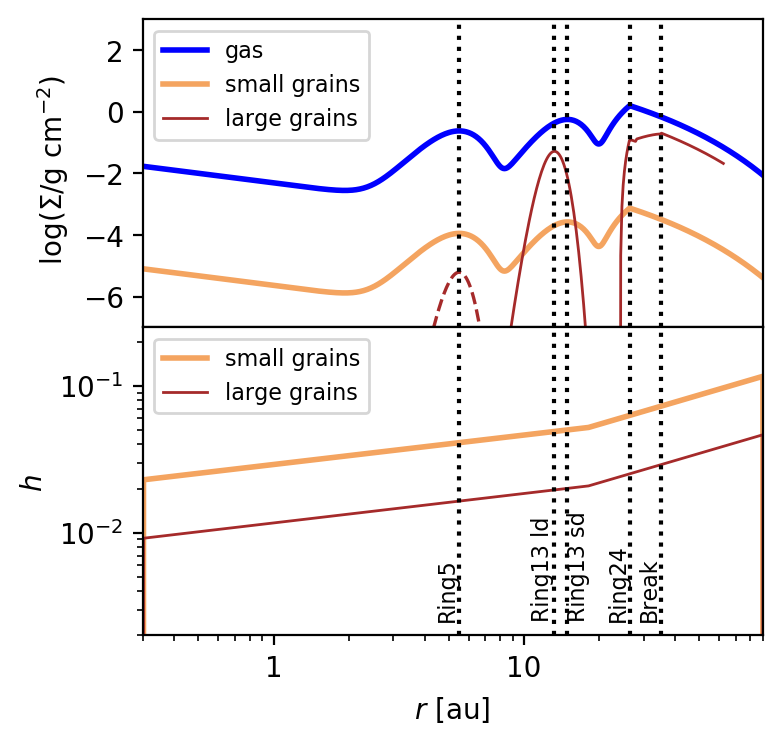
\includegraphics[width=\columnwidth]{allprofiles.png}
    \caption{Top panel shows the surface density profiles for the gas, the large and small grain populations. Bottom panel shows the scale height $h(r)$ as a function of polar radius. The dashed lines crossing both panels are the radii that confine the structures.}
    \label{fig:profiles}
\end{figure}

The final structure of the parametric model goes as Fig. \ref{fig:profiles} shows. The inner radius of the model grid was set to 0.1\,au and an otter radius of 115\,au, large enough for the dust disc to become undetectable.

The dust begins at 0.3\,au, out of the zone expected to be cleared by dynamical interactions with the central binary \citep{Art_Lu}. For the small dust grains, we propose a three ringed structure. The innermost ring of the model is located from 5 to 8\,au ,this ring is not present in the observations but was added for having a better SED fit. Then follows the two observed rings: the first goes from 12 to 19.5\,au and, with a 1\,au-wide gap between them, the outer ring goes from 20.5\,au and has its maximum density peak at 25\,au. The small-dust density then then fades as the radius increases.

On the other hand, in order to reproduce the two ringed observed morphology of the millimetre continuum emission we required a model that has its large-dust grain population distributed with a wide central cavity (r = 12.3\,au), a narrow 2.6\,au-wide inner ring followed by a gap of 8.2\,au that separates both rings and then an outer ring that goes from 23\,au and has it density peak at 27.3\,au. This last ring has a break between 32 and 34.5\,au and then reaches out to 57\,au.

For the vertical structure, \citet{dOrazi} found flaring angles of $\varphi$ = 6.2$\pm$0.6\,$\degr$ for the inner ring and $\varphi$ = 8.5$\pm$1.0\,$\degr$ for the outer one. For that matter, we used two different flaring index $\psi$ for our model. The separation between the two values was set at $r$ = 19\,au with values of 0.2 and 0.5 for the inner part and the outer part respectively. Also, the scale height is calculated using $H_o$ = 0.045 and $r_0$ = 19.5\,au.

We set the values of the inclination an the position angle as the same as those obtained from the ALMA observation in Section \ref{sec:Observations}, so the model has an inclination of i = 33.9\,$\degr$ and a P.A. = 74.6\,$\degr$. Finally, we set the distance at d = 72.4\,pc \citep{Gaia}.

\section{Model results and discussion} \label{sec:results}

Our parametric model is fairly successful in reproducing the available data. The simulated images and the SED of the model
are shown in Fig. \ref{fig:two} and Fig. \ref{fig:SED} respectively.

The simulated image at 1.65\,$\micron$ shows a similar radial structure to the one visible in the observations displaying a two ringed disc, where the innermost small-dust ring of the parametric model hides under the artificial coronagraph. The visible asymmetry in the SPHERE observations is recreated using grains larger than 0.4\,$\micron$ as smaller grains do not cause a strong forward scattering, meaning that the disc is depleted of very-small grains. Interestingly, the model accurately shows the shadows described by \citet{dOrazi} that are present in the Sphere-IRDIS image.

The simulated 1.3\,mm continuum image displays some clear similarities with the ALMA observation. The model reproduced the two rings that are present in the observation: the faint inner ring and the outer brighter one. %The outer ring has an intensity peak at $\sim$30\,au and a break present at $\sim$35\,au. 
As the radial profiles obtained from the simulated images of the model closely resemble those deduced from the observations (Fig. \ref{fig:radprofiles}), we can assume that the model provides a reliable approximation of the disc structure, including, particularly for our interest, the dimensions of the previously unseen 1.3\,mm thin inner ring. Accordingly, taking the parametric model values for the large-dust inner ring we can have that it is located at 13.6\,au, has an estimated width of 2.6\,au, an estimated scale height ranging from 0.25 to 0.32\,au and a dust mass of about 3\,M$_{\earth}$.

As \citet{2018ApJ...869L..46D} explains, the stability of a narrow dust ring can be analysed comparing its height to its radial extent. For a ring to be stable and long-lived its horizontal dimension can not be less than its vertical height. Using the parametric model scale height of 0.28\,au at 13.46\,au and the measured width of the inner ring (4.17\,au, see Section \ref{sec:Observations}), we have that its width is $\sim$15 times its scale height, meaning that it is stable and the disc is capable of supporting a thin ring as this one.

Fig. \ref{fig:SED} shows the SED constructed from the model compared to the photometry data available in the literature in \citet{Jensen_97} and online in \textsc{vizier} and \textsc{diana}, and also using spectrometry data from an archival \textit{Spitzer} IRS spectrum. From the similarity between the data and the resulting SED of the model we confirm that there has to be a small-grain population close to the stars down to 0.3\,au. The decision of employing the three ringed structure for the small dust grains relies on the fact that the SED needed a ring at a radius smaller than 10\,au to have a proper fit, this proposed ring has not been observed. The unexpected central emission in the 1.3\,mm continuum image could be part of this inner ring and, as it is asymmetric, the ring could be lopsided.

\begin{figure}
	\centering
	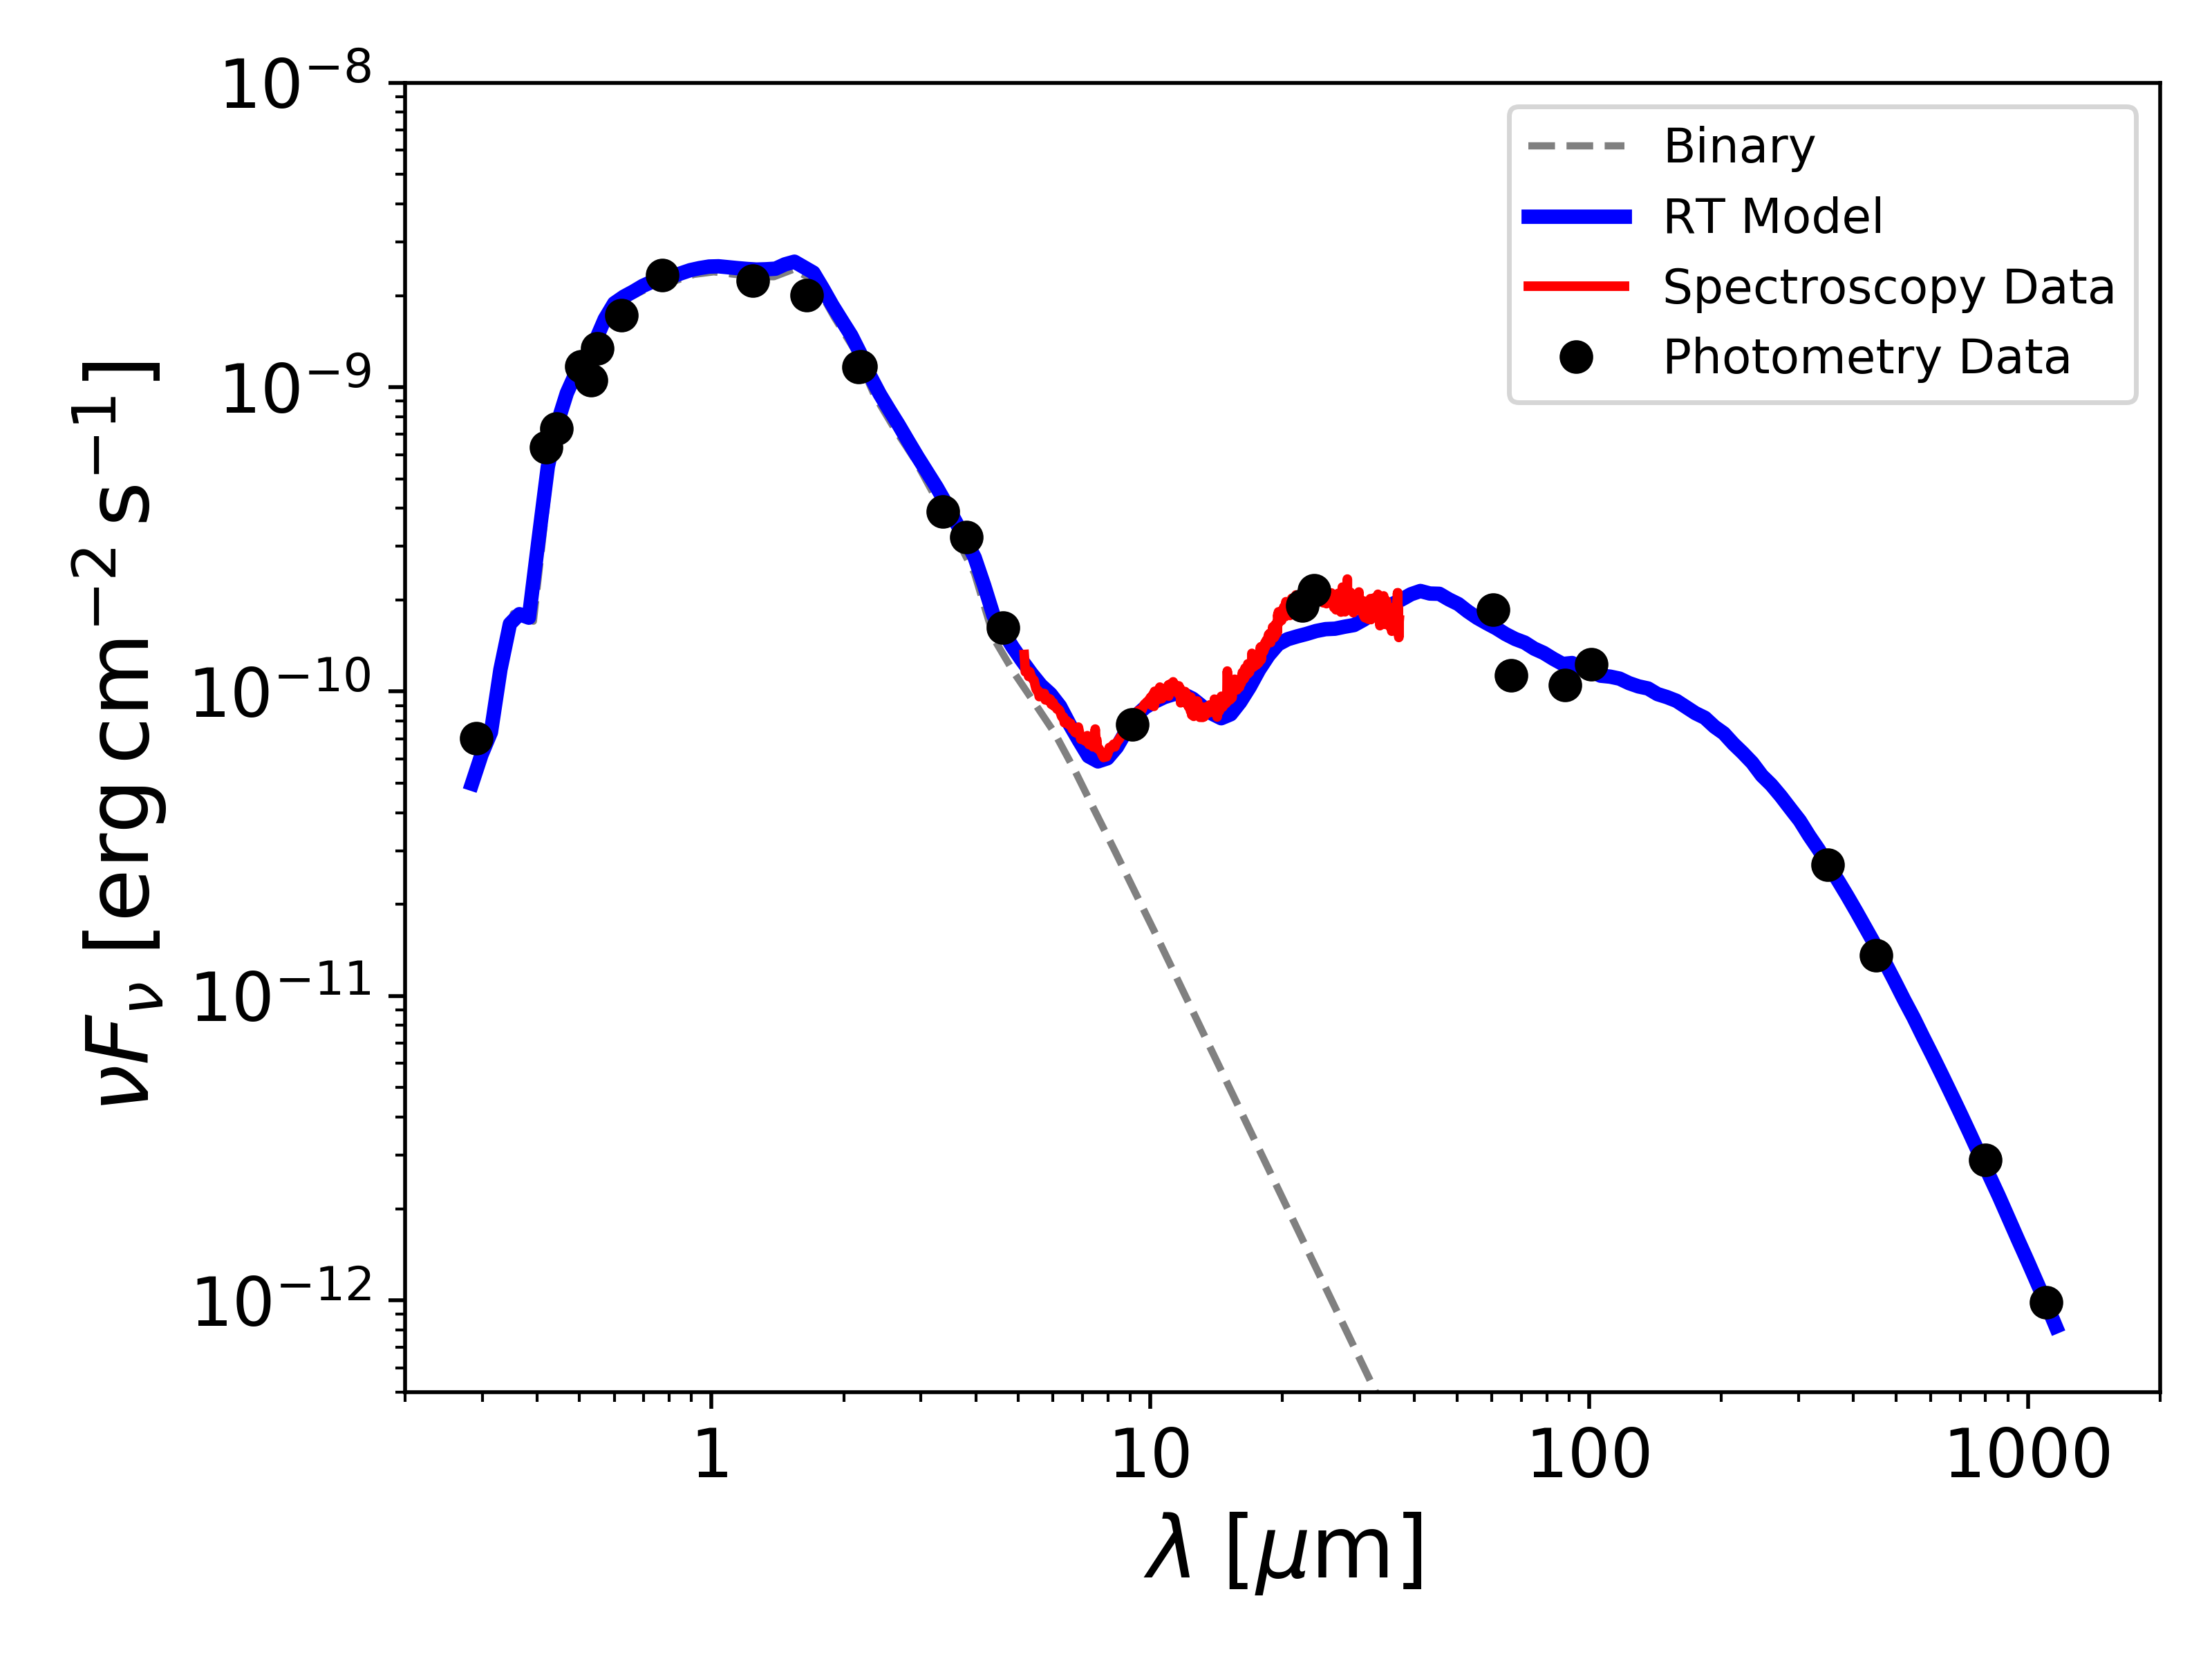
\includegraphics[width=\columnwidth]{SED_.png}
    \caption{The SED (black points and solid red curve) compared with the model (blue). The black points represent the measured photometry and the red line shows an archival \textit{Spitzer} IRS spectrum.}
    \label{fig:SED}
\end{figure}


%\begin{table}
% \caption{Model rings masses}
% \label{tab:masses}
% \begin{tabular}{lcc}
%  \hline
%  Ring & Location & Mass\\
%   & $\mathrm{au}$ & $M_{\earth}$ \\
%  \hline
%  First & 5 to 8 & 0.0007 \\
%  Second & 11 to 19 & 2.9 \\
%  Third & 20 to 80 & 43 \\
%  \hline
% \end{tabular}
%\end{table}


\section{Conclusions} \label{sec:Conclusions}

New ALMA 1.3\,mm continuum imaging of the circumbinary disc around V4046\,Sgr reveals new information about its substructure. Using a radiative transfer model, a preexisting scattered light observation and decompositions in polar coordinates of the computed \textsc{uvmem} model image, we measured and analysed the previously unseen thin inner ring and studied the small-dust population distribution.

The key conclusions of our analysis are as follows.
\begin{itemize}
  \item We report a narrow inner ring for the 1.3\,mm continuum located at 13.46$\pm$0.43\,au from the stars and has an estimated width of 4.17$\pm$0.94\,au. The location of this ring is similar to the inner ring observed in the scattered light image, this reveals that the ring includes a considerable mass of millimetre-sized grains of around 3\,M$_{\earth}$. Using the parametric model scale height value ($h= $ 0.28\,au at 13.46\,au) we have that the ring width is $\sim$15 times its estimated height, making it a stable ring.
  
  \item The 1.3\,mm outer ring, that starts at $\sim$23\,au and has its peak intensity at $\sim$32\,au, presents a visible break in the surface brightness at $\sim$35\,au. 
  
  %\item The inner ring may not be totally resolved as its width is comparable to the beam size. Future observation with smaller beams sizes could give an answer on the real radial extent of the ring.
  
  \item We interpret the asymmetry observed with SPHERE-IRDIS at 1.65\,$\micron$ due to strong forward-scattering, which implies that the dust population is depleted of grains smaller than $\sim$0.4\,$\micron$.
  
  \item As our parametric model accounts for the SED of the system, the disc requires the existence of a sub-micron dust population close (<5\,au) to the stars. We also predict the existence of another thin ring at $\sim$6\,au, about 3\,au-wide and made of small dust grains that lies under the coronagraph of the SPHERE images. Additionally, the weak central emission at 1.3\,mm could be part of this ring.
  
\end{itemize}

Finally, we encourage additional detailed analysis and more modelling that could give some explanations of the substructures present on the disc. Higher resolution observations of radio continuum may provide the opportunity to make better measurements of the rings radial extension. For future radiative transfer models, it might be worth adding gas, using different inclinations for the inner and outer disc and implementing hydrodynamic simulations too, especially to try to unravel the mystery of how the inner ring is so thin an stable. 

\section*{Acknowledgements}

Try to keep it short.

\section*{Data Availability}

%%%%%%%%%%%%%%%%%%%% REFERENCES %%%%%%%%%%%%%%%%%%

% The best way to enter references is to use BibTeX:

\bibliographystyle{mnras}
\bibliography{bibtex} % if your bibtex file is called example.bib


% Alternatively you could enter them by hand, like this:
% This method is tedious and prone to error if you have lots of references
%\begin{thebibliography}{99}
%\bibitem[\protect\citeauthoryear{Author}{2012}]{Author2012}
%Author A.~N., 2013, Journal of Improbable Astronomy, 1, 1
%\bibitem[\protect\citeauthoryear{Others}{2013}]{Others2013}
%Others S., 2012, Journal of Interesting Stuff, 17, 198
%\end{thebibliography}

%%%%%%%%%%%%%%%%%%%%%%%%%%%%%%%%%%%%%%%%%%%%%%%%%%

%%%%%%%%%%%%%%%%% APPENDICES %%%%%%%%%%%%%%%%%%%%%

%%%%%%%%%%%%%%%%%%%%%%%%%%%%%%%%%%%%%%%%%%%%%%%%%%


% Don't change these lines
\bsp	% typesetting comment
\label{lastpage}
\end{document}

% End of mnras_template.tex
